\documentclass{beamer}
\usecolortheme{crane}
\usepackage{xspace}
\usepackage{stackengine}
\usepackage{amssymb}
\usepackage{graphicx}
\usepackage{tikz}
\usepackage{pgfplots}
\pgfplotsset{width=10cm,compat=1.9}

\newcommand{\diamonddash}{\ensurestackMath{%
  \stackengine{.5pt}{\diamond}{\scalebox{.4}[.85]{$-$}}{O}{c}{F}{F}{L}}}

\setbeamertemplate{navigation symbols}{}
\setbeamertemplate{blocks}[rounded][shadow=false]

\newtheorem{remark}[theorem]{Remark}
\newtheorem{property}[theorem]{Property}

\title{Runtime Verification For Android Security}
\author{Richard Allen\\Swansea University, UK}
\date{Viva 13 December 2021}

\begin{document}

% Title

\frame{\titlepage}

%% Contents
%
%\frame{
%\vfill
%\begin{block}{}
%\begin{center}
% \mbox{ } \\
%{\huge Contents}
%\mbox{ } \\
%\end{center}
%\end{block}
%\vfill
%Monitoring For Collusion\\
%Monitoring With the Rosu-Havelund Algorithm\\
%Monitoring With the Reverse Rosu-Havelund Algorithm\\
%\vfill
%}

%  Say I know you have read my dissertation and I would like to highlight the main points and give a practical demonstration of my implementation.

\frame{
\vfill
\begin{block}{}
\begin{center}
 \mbox{ } \\
{\huge Monitoring For Collusion}
\mbox{ } \\
\end{center}
\end{block}
\vfill
}

% Background 
% Android Security

\frame{\frametitle{Why Is Android Security An Important Topic?}

\vfill

\begin{itemize}

\item In 2019 there is reported 3.4 billion smart phone users world wide\footnote{https://www.statista.com/statistics/330695/number-of-smartphone-users-worldwide/}, 1.6 billion are Android devices\footnote{https://www.statista.com/statistics/543185/worldwide-internet-connected-operating-system-population/}.

\item Attacks happen to such extent that the McAfee Q1 2020 threat reports opens with the headline “Mobile Malware Is Playing Hide and Steal”\footnote{https://www.mcafee.com/content/dam/consumer/en-us/docs/2020-Mobile-Threat-Report.pdf}.

\item We are monitoring for security on one concrete example: app collusion for information theft.
 
\end{itemize}

}
%
%\frame{\frametitle{What Is the Android Security Concept?}
%
%\begin{figure}[h]
%  \centering
%  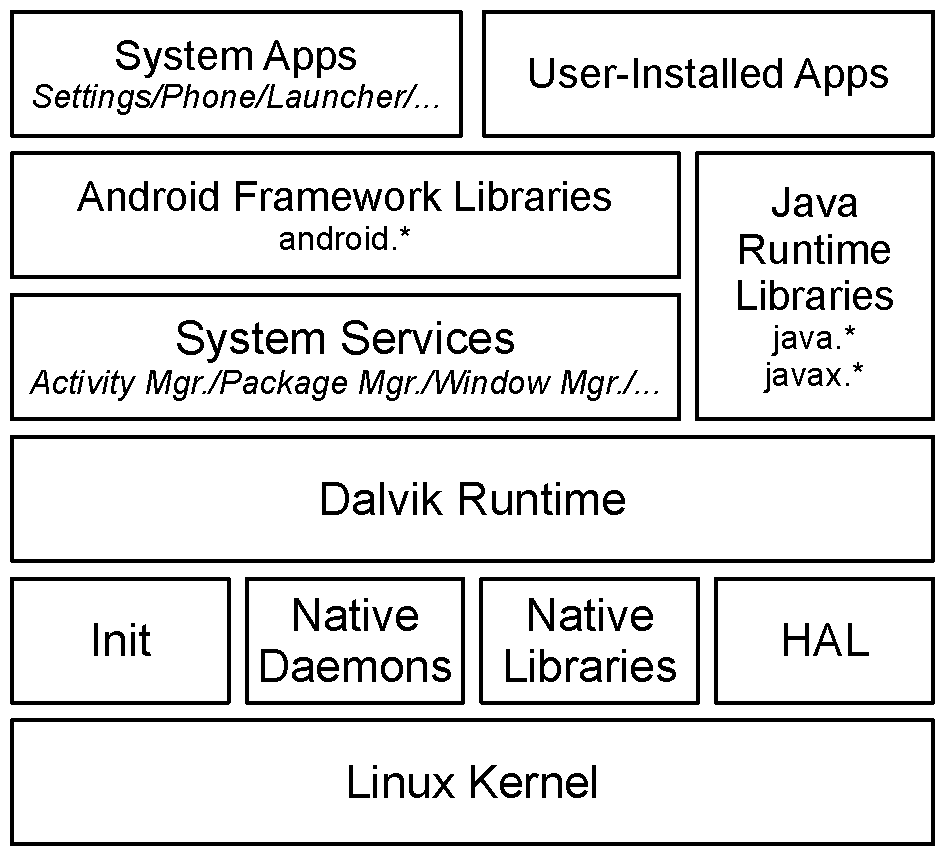
\includegraphics[width=0.4\textwidth]{AndroidStack.pdf}
%\end{figure}
%
%\begin{itemize}
%
%\item Linux Kernel separates processes into sandboxes where they are unable to reference each others address space directly.
%
%\item Android restricts access to sensitive resources to only those applications that have been granted permission by the user.
%
%\item Applications can communicate with each other to enhance features but this can be exploited to share permissions.
%
%\end{itemize}
%
%}

\frame{\frametitle{Collusion: Specific Attack On Android}

By collusion we mean where two or more applications communicate between themselves in order to use their combined permissions to perform malicious activities like stealing information.  

This was theorised at least as early as 2011 and found to be occurring in 2017 \footnote{J. Blasco, T. Chen, I. Muttik, and M. Roggenbach.  Detection of app collusion potential using logic programming.  Journal of Network and Computer Applications, 105, 06 2017}.
  
\begin{figure}[h]
  \centering
  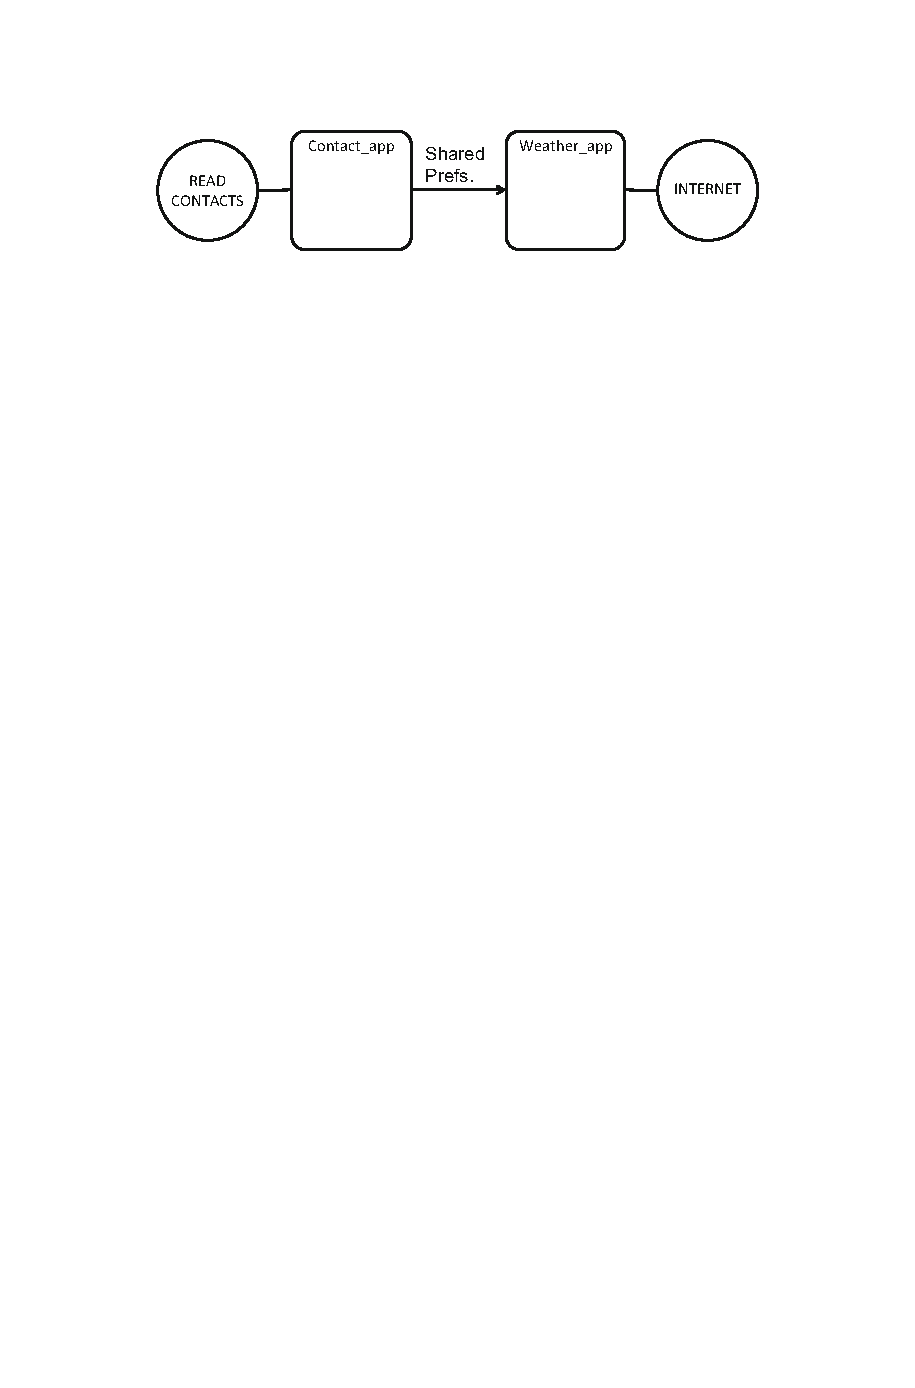
\includegraphics[width=0.7\textwidth]{Collusion.pdf}
\end{figure}

}

%\frame{\frametitle{App Collusion and Operating System Calls}
%  
%General Definition\footnote{Asavoae et al: Detecting Malicious Collusion Between Mobile Software.  Applications: The Android Case.  Data Analytics and Decision Support for Cybersecurity, Springer 2017}:  There is a non-singleton set S of apps performing a threat such that:
%
%\begin{itemize}
%
%\item Each app in S contributes the execution of at least one action to the threat.
%\item Each app in S communicates with at least one other app. 
%
%\end{itemize}
%\vfill
%
%Observation:
%
%\begin{itemize}
%
%\item Accessing protected resources in Android (actions) and
%\item communication 
%
%\end{itemize}
%
%require operating system calls.
%
%}
%
\frame{\frametitle{Intercepting Operating System Calls in Android}

\underline{Xposed Framework\footnote{First released in 2012 by rovo89}:}

\begin{itemize}

\item Modifies the Linux Zygote process from which all processes are forked.
\item This allows us to intercept operating system calls made by all processes.

\end{itemize}
\vfill
  
\begin{figure}[h]
  \centering
  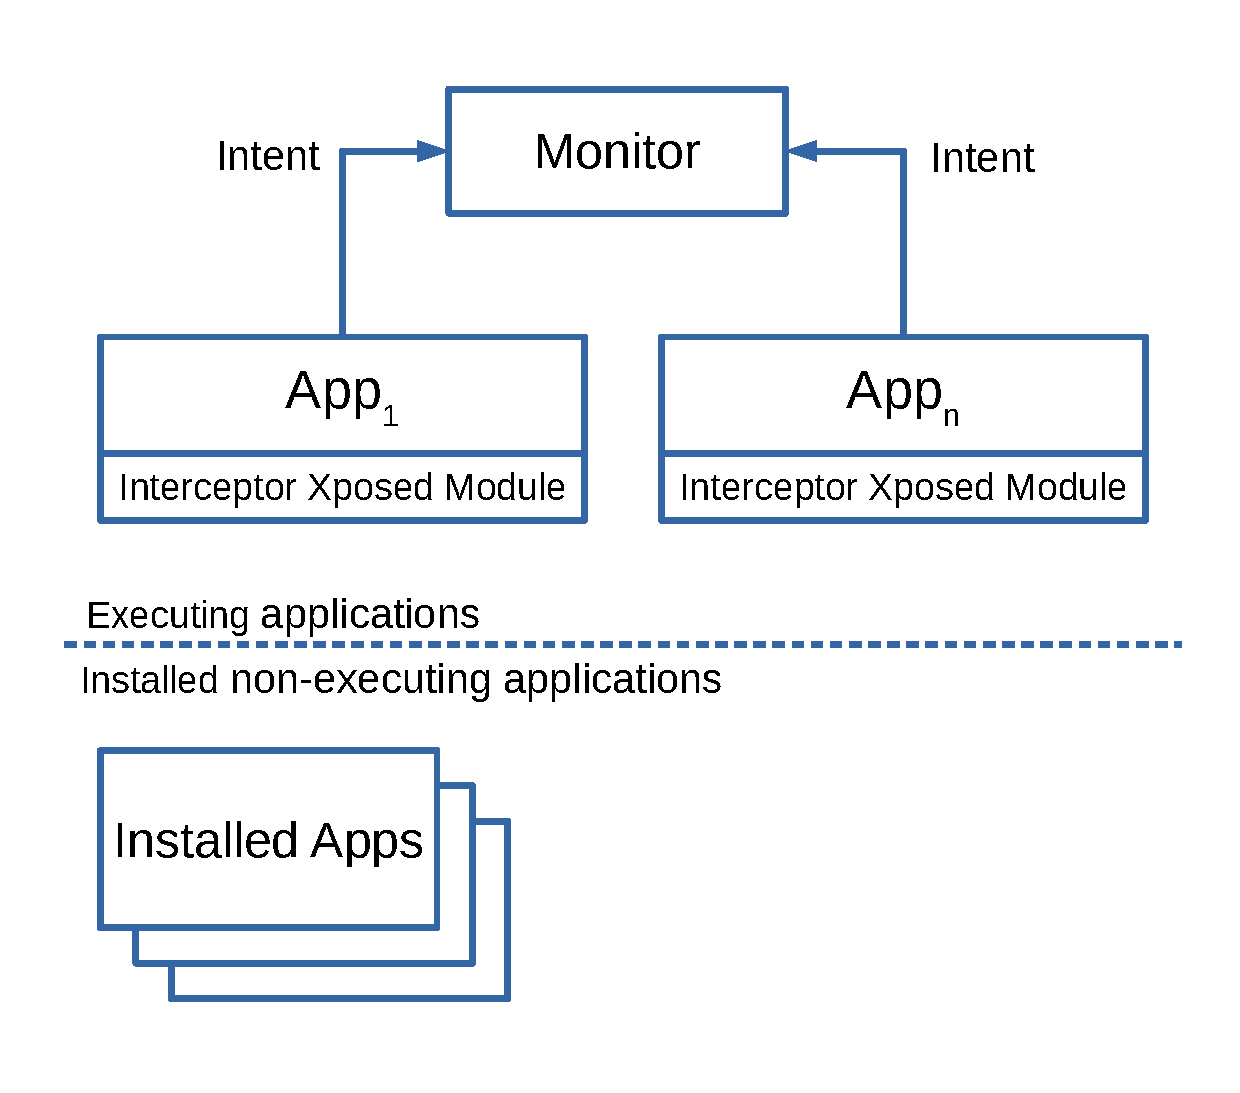
\includegraphics[width=0.4\textwidth]{HighLevelArchitecture2.pdf}\\
  \underline{Our Implemented Monitoring Architecture}
\end{figure}  
  
}

\frame{
\vfill
\begin{block}{}
\begin{center}
 \mbox{ } \\
{\huge Monitoring With the Rosu-Havelund Algorithm}
\mbox{ } \\
\end{center}
\end{block}
\vfill
}

\frame{\frametitle{Rosu-Havelund Algorithm}

We attempted to use the Rosu-Havelund Algorithm \footnote{Grigore Rosu and Klaus Havelund.  Synthesizing Dynamic Programming Algorithms from Linear Temporal Logic Formulae.  RIACS, 2001} as an alternative to Buchi automata to evaluate LTL over a trace.

\begin{itemize}

\item Uses logic of the `future', i.e, Always $\square$, Eventually $\diamond$, Next $\circ$, Until $U$.
\item Collusion For Information Theft between two apps: $\diamond(q \land (\diamond s \land (\diamond r \land (\diamond p ))))$.
\item Traverses the trace from the latest event to the earliest to implement future operators.
\item Each time an event occurs the trace grows and the computational steps to evaluate the trace increases.
\item We theorise the number of computational steps follows n(n+1)/2, therefore the complexity is $O(n^2 * |\varphi|)$ where $n$ is the number of events in the trace and $\varphi$ is the size of the formula.
\end{itemize}

}

\frame{\frametitle{Complexity Analysis}

Given the collusion formula we measured:
 
%\begin{table}[h!]
%	\centering
\begin{center}
	\begin{tikzpicture}[scale=0.7, every node/.style={transform shape}]
	\begin{axis}[
	    xlabel={Trace Length [events]},
	    ylabel={Duration [seconds]},
	    xmin=10, xmax=100,
	    ymin=0, ymax=1500,
	    xtick={10,20,30,40,50,60,70,80,90,100},
	    ytick={0,100,200,300,400,500,600,700,800,900,1000,1100,1200,1300,1400,1500},
	    legend pos=south east,
	    ymajorgrids=true,
	    grid style=dashed,
	]
	
	\addplot[
	    color=blue,
	    mark=square,
	    ]
	    coordinates {
	    (10,17)(20,72)(30,145)(40,203)(50,326)(60,462)(70,692)(80,941)(90,1198)(100,1449)
	    };
	    \addlegendentry{Standard Rosu-Havelund}
	    
	\addplot[
	    domain=0:100, 
	    samples=20, 
	    color=red,
	    mark=triangle,
	    ]
	    {(x * (x+1)) / 2};
	    \addlegendentry{n(n+1)/2}    
	\end{axis}
	\end{tikzpicture}
\end{center}
%	\caption{Dependency Between Trace Length and Evaluation Duration}
%	\label{tab:StandardRHEvaluationDuration}
%\end{table}

This makes the algorithm unsuitable for realtime monitoring.

}

% Contribution 

\frame{
\vfill
\begin{block}{}
\begin{center}
 \mbox{ } \\
{\huge Monitoring With the Reverse Rosu-Havelund Algorithm}
\mbox{ } \\
\end{center}
\end{block}
\vfill
}

\frame{\frametitle{Reverse Rosu-Havelund Algorithm}

\begin{itemize}

\item Traverses the traces in the opposite direction to standard R/H algorithm.

\item Reduces complexity in realtime monitoring by reusing the result of the previous evaluation, therefore only the latest event has to be evaluated.

\item Comes at the expense that the LTL operators that deal with future events (next, eventually) cannot be implemented because we do not know what future events will be.  Operators that are concerned with past events are implemented (previous, once) instead.

\item Collusion property expressed with past operators: $$ \diamonddash(p \land \diamonddash(r \land \diamonddash(s \land \diamonddash q))) $$

\end{itemize}

}

%\frame{\frametitle{Collusion Property in LTL with the Once operator}
%
%The Once, \diamonddash, operator described by Pnueli\footnote{Zohar Manna, Amir Pnueli.  The Temporal Logic of Reactive and Concurrent Systems.  Springer-Verlag 1992} holds if an event has occurred in the present or at some preceding time.
%
%\begin{itemize}
%
%\item Once semantics:  $(\sigma, j) \models \diamonddash p\ iff\ (\sigma, k) \models p\ for\ some\ k,\ 0 \leq k \leq j$.
%\item Eventually semantics, for comparison:  $(\sigma, j) \models \diamond p\ iff\ (\sigma, k) \models p\ for\ some\ k,\ k \geq j$.
%
%\end{itemize}
%
%}

%\frame{\frametitle{}
%
%\begin{itemize}
%
%\item Our collusion property looks for a \underline{p}ublish event, preceded by a \underline{r}eceive event, preceded by a \underline{s}end event, preceded by a \underline{q}uery event.\\
%
%\end{itemize}
%
%\begin{center}
%
%$ \diamonddash(p \land \diamonddash(r \land \diamonddash(s \land \diamonddash q))) $
%
%\end{center}
%
%}

%\frame{\frametitle{Conjecture}
%
%\begin{itemize}
%
%\item Security properties can always be described in terms of past events because we are looking for when a security policy \textit{has} been broken.
%
%\item For instance, a policy might be that there should be no audio taken from the microphone if there are no calls in progress.
%
%\item In that case we would look for an audio read event to have taken place with no preceding call events.
%
%\item Pneuli describes the past temporal operators as `a symmetric counterpart to each of the future operators.  While the future formula describes a property holding at a suffix of the model (...), a past formula describes a property of a prefix of the model' 
% 
%\end{itemize}
%  
%}

\frame{\frametitle{Complexity}

Given the collusion formula we measured:

%\begin{table}[h!]
%	\centering
\begin{center}
	\begin{tikzpicture}[scale=0.7, every node/.style={transform shape}]
	\begin{axis}[
	    xlabel={Trace Length [events]},
	    ylabel={Duration [seconds]},
	    xmin=10, xmax=100,
	    ymin=0, ymax=1500,
	    xtick={10,20,30,40,50,60,70,80,90,100},
	    ytick={0,100,200,300,400,500,600,700,800,900,1000,1100,1200,1300,1400,1500},
	    legend pos=south east,
	    ymajorgrids=true,
	    grid style=dashed,
	]
	
	\addplot[
	    color=blue,
	    mark=square,
	    ]
	    coordinates {
	    (10,17)(20,72)(30,145)(40,203)(50,326)(60,462)(70,692)(80,941)(90,1198)(100,1449)
	    };
	    \addlegendentry{Standard R-H}
	    
	\addplot[
	    color=green,
	    mark=diamond,
	    ]
	    coordinates {
	    (10,1)(20,1)(30,1)(40,1)(50,1)(60,1)(70,1)(80,1)(90,1)(100,1)
	    };
		\addlegendentry{Reverse R-H}
	\end{axis}
	\end{tikzpicture}
\end{center}
%	\caption{Dependency Between Trace Length and Evaluation Duration}
%	\label{tab:ReverseRHEvaluationDuration}
%\end{table}

Suitable for realtime monitoring: takes in the order of $\leq$10ms per new event.

}

\frame{\frametitle{Live Demo}

\begin{figure}[h]
\centering
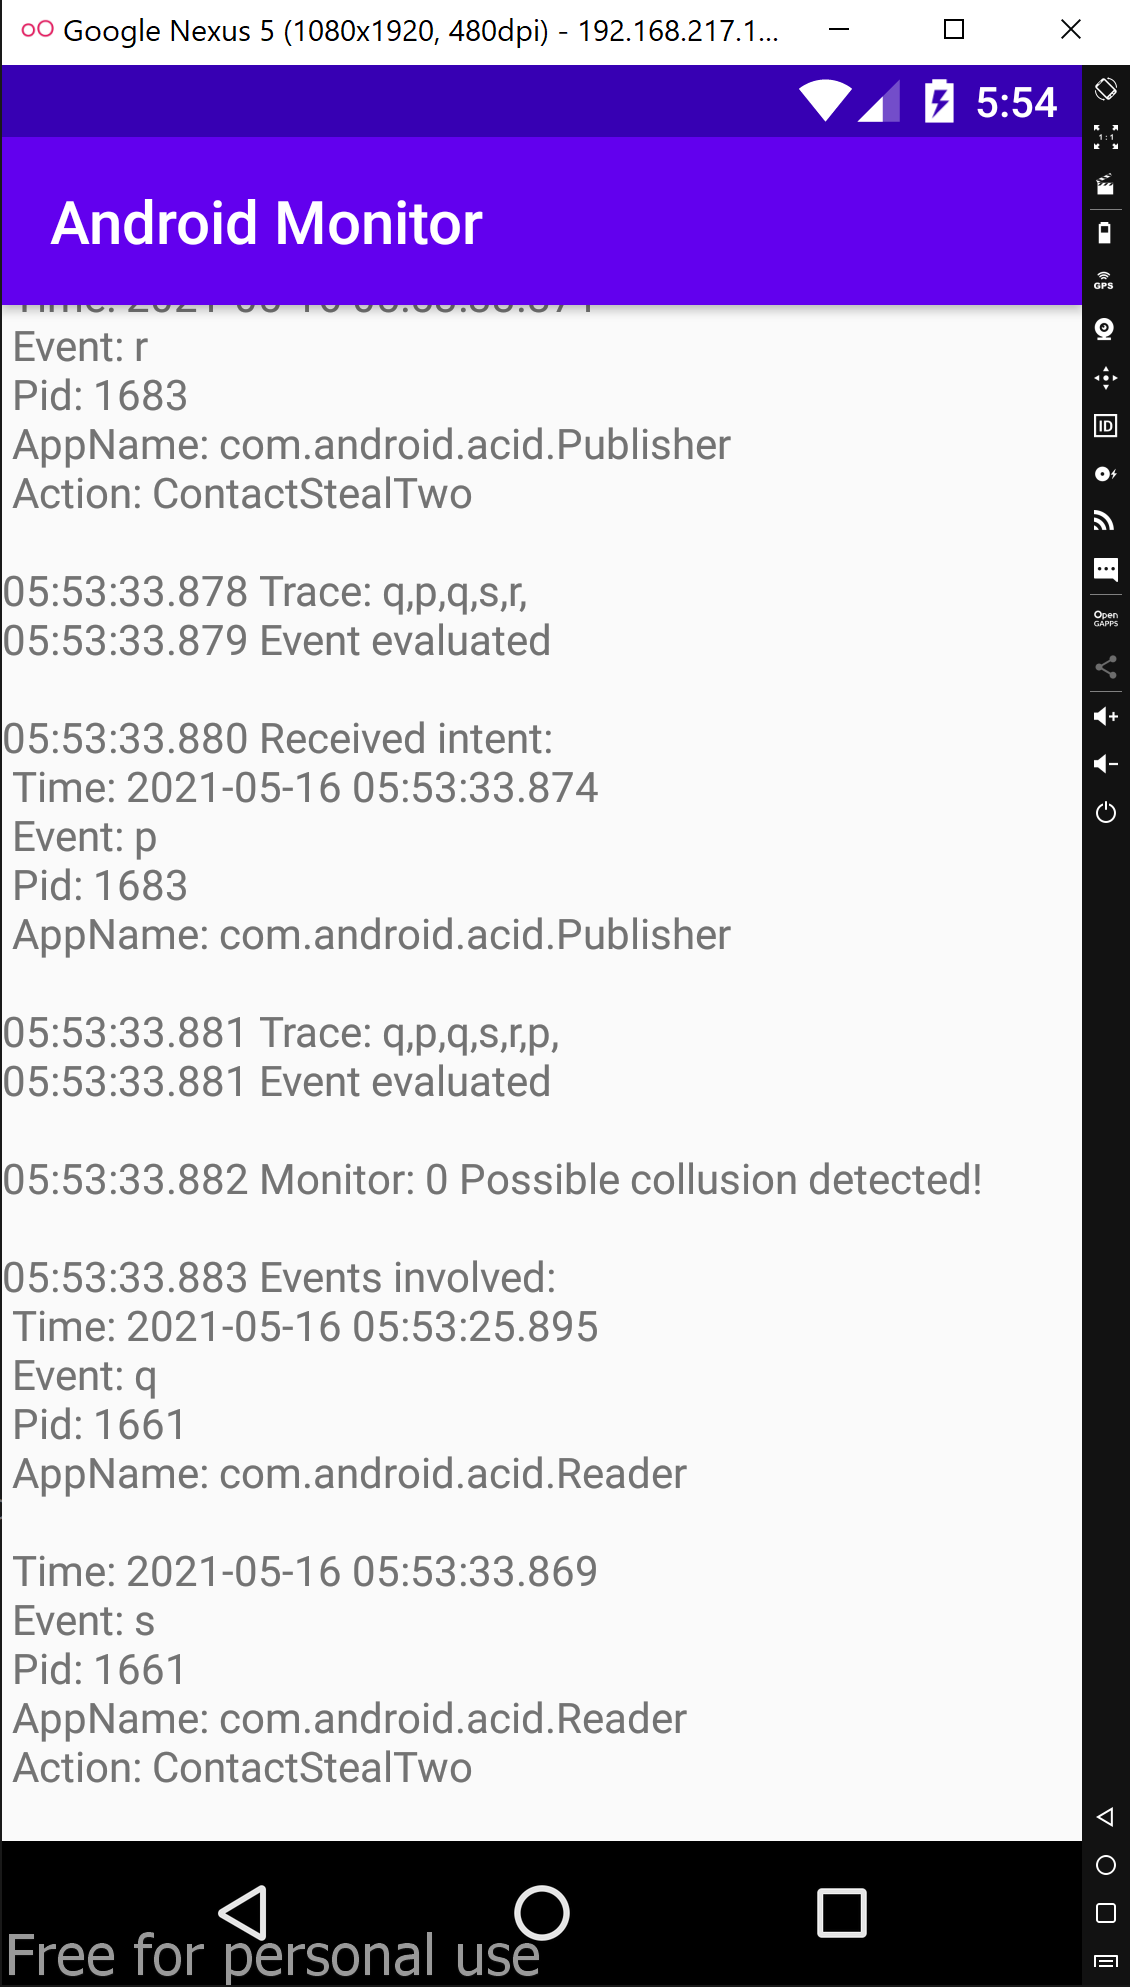
\includegraphics[width=0.4\textwidth]{MonitorScreenshot.png}
\end{figure}
   
}

\frame{\frametitle{Runtime Monitoring For Security (Collusion) In Context}

\vfill

\begin{itemize}

\item Model checking apps has false positives (over approximation), works for small apps only\footnote{\tiny Software Model Checking for Mobile Security(...).  Irina Mariuca Asavoae, Hoang Nga Nguyen, Markus Roggenbach.  SPIN 2018: 3-25}. 

\item Static analysis has false positives (no reachability analysis)\footnote{\tiny Detection of app collusion potential using logic programming.  Jorge Blasco, Thomas M. Chen, Igor Muttik, Markus Roggenbach.  J. Netw. Comput. Appli. 105: 88-104 (2018)}.  

\item Machine learning has false positive and false negatives\footnote{\tiny Towards a threat assessment framework for apps collusion.  Kalutarage, Harsha Kumara and Nguyen, Hoang Nga and Shaikh, Siraj Ahmed.  Telecommunication Systems.  Springer US 2017: 1-14}.

\end{itemize}

\vfill

\begin{center}
\textit{\large Runtime monitoring is effective!} %has false positives (no checks for metadata), is effective. 
\end{center}

\vfill

Based on the positive results of my project, Swansea University and Coventry University are applying for funding for monitoring for security in an Innovate UK call.

}

%\frame{
%\vfill
%\begin{block}{}
%\begin{center}
% \mbox{ } \\
%{\huge Conclusion}
%\mbox{ } \\
%\end{center}
%\end{block}
%\vfill
%}
%
%\frame{\frametitle{Summary}
%
%\begin{itemize}
%
%\item Monitoring for Android security is possible.
%
%\item Requires "logic of the past".
%
%\item It is useful to monitor on abstract events.
%
%\end{itemize}
%
%It is possible to monitor for collusion without false positives if we restrict collusion to attempts within a limited timeframe.
%
%}
%
%\frame{\frametitle{Future Work}
%
%\begin{itemize}
%
%\item Systematic experimentation with the monitors.
%
%\item Monitor for more properties e.g. use of the camera or microphone.
%
%\item Extend the grammar and semantics of LTL to evaluate properties looking for collusion involving more than 2 apps.
%
%\item Evaluation of future operators by adapting the algorithm to use a three-valued variation of LTL, similar to the logic of Bauer et al.\\
%
%\item Investigate if deriving monitors for concrete events from monitors for abstract events leads to better results than using monitors derived from LTLFO.
%
%\item Cover more Android versions, integrate Xposed framework into monitor, provide a security monitoring app.
%
%\end{itemize}
%
%%\begin{verbatim}
%%
%%      Propositional LTL                          FOL LTL
%%          |                                                   |
%%          v                                                  v
%%     monitor        monitor                    monitor
%%     abstract  ->  conrete I                  concrete II (competitors do)
%%
%%\end{verbatim}
%
%}

\end{document}